% Figure from MATH 591 notes, section 68. After the board (Lecture 24): the uniform time lemma cartoon.
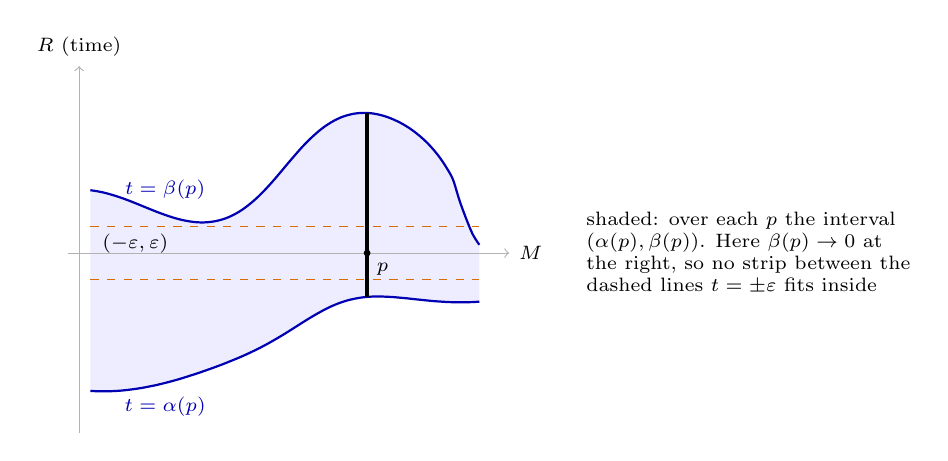
\begin{tikzpicture}[scale=0.95]
\fill[blue!7] plot[smooth] coordinates {(-2.600,0.840) (-2.512,0.827) (-2.424,0.809) (-2.336,0.786) (-2.247,0.759) (-2.159,0.729) (-2.071,0.696) (-1.983,0.661) (-1.895,0.625) (-1.807,0.589) (-1.719,0.554) (-1.631,0.521) (-1.542,0.490) (-1.454,0.463) (-1.366,0.441) (-1.278,0.424) (-1.190,0.413) (-1.102,0.409) (-1.014,0.414) (-0.925,0.427) (-0.837,0.449) (-0.749,0.481) (-0.661,0.524) (-0.573,0.577) (-0.485,0.642) (-0.397,0.716) (-0.308,0.801) (-0.220,0.894) (-0.132,0.993) (-0.044,1.097) (0.044,1.202) (0.132,1.305) (0.220,1.405) (0.308,1.497) (0.397,1.581) (0.485,1.656) (0.573,1.719) (0.661,1.771) (0.749,1.813) (0.837,1.843) (0.925,1.863) (1.014,1.873) (1.102,1.873) (1.190,1.864) (1.278,1.846) (1.366,1.820) (1.454,1.785) (1.542,1.743) (1.631,1.692) (1.719,1.632) (1.807,1.562) (1.895,1.482) (1.983,1.387) (2.071,1.277) (2.159,1.145) (2.247,0.985) (2.336,0.700) (2.424,0.460) (2.512,0.250) (2.600,0.110)} -- plot[smooth] coordinates {(2.600,-0.650) (2.512,-0.655) (2.424,-0.658) (2.336,-0.659) (2.247,-0.657) (2.159,-0.654) (2.071,-0.648) (1.983,-0.642) (1.895,-0.633) (1.807,-0.624) (1.719,-0.615) (1.631,-0.605) (1.542,-0.597) (1.454,-0.589) (1.366,-0.584) (1.278,-0.581) (1.190,-0.581) (1.102,-0.586) (1.014,-0.596) (0.925,-0.612) (0.837,-0.633) (0.749,-0.661) (0.661,-0.695) (0.573,-0.735) (0.485,-0.781) (0.397,-0.831) (0.308,-0.884) (0.220,-0.939) (0.132,-0.995) (0.044,-1.051) (-0.044,-1.105) (-0.132,-1.157) (-0.220,-1.207) (-0.308,-1.254) (-0.397,-1.299) (-0.485,-1.341) (-0.573,-1.381) (-0.661,-1.418) (-0.749,-1.454) (-0.837,-1.489) (-0.925,-1.522) (-1.014,-1.554) (-1.102,-1.585) (-1.190,-1.615) (-1.278,-1.643) (-1.366,-1.671) (-1.454,-1.697) (-1.542,-1.721) (-1.631,-1.744) (-1.719,-1.765) (-1.807,-1.783) (-1.895,-1.800) (-1.983,-1.814) (-2.071,-1.826) (-2.159,-1.836) (-2.247,-1.843) (-2.336,-1.847) (-2.424,-1.848) (-2.512,-1.847) (-2.600,-1.843)} -- cycle;
\draw[orange!85!black, dashed] (-2.6,-0.35) -- (2.6,-0.35); \draw[orange!85!black, dashed] (-2.6,0.35) -- (2.6,0.35);
\draw[->, gray!60] (-2.9,0) -- (3.0,0) node[right, font=\scriptsize, text=black] {$M$};
\draw[->, gray!60] (-2.75,-2.4) -- (-2.75,2.5) node[above, font=\scriptsize, text=black] {$\mathbb{R}$ (time)};
\draw[blue!70!black, thick] plot[smooth] coordinates {(-2.600,0.840) (-2.512,0.827) (-2.424,0.809) (-2.336,0.786) (-2.247,0.759) (-2.159,0.729) (-2.071,0.696) (-1.983,0.661) (-1.895,0.625) (-1.807,0.589) (-1.719,0.554) (-1.631,0.521) (-1.542,0.490) (-1.454,0.463) (-1.366,0.441) (-1.278,0.424) (-1.190,0.413) (-1.102,0.409) (-1.014,0.414) (-0.925,0.427) (-0.837,0.449) (-0.749,0.481) (-0.661,0.524) (-0.573,0.577) (-0.485,0.642) (-0.397,0.716) (-0.308,0.801) (-0.220,0.894) (-0.132,0.993) (-0.044,1.097) (0.044,1.202) (0.132,1.305) (0.220,1.405) (0.308,1.497) (0.397,1.581) (0.485,1.656) (0.573,1.719) (0.661,1.771) (0.749,1.813) (0.837,1.843) (0.925,1.863) (1.014,1.873) (1.102,1.873) (1.190,1.864) (1.278,1.846) (1.366,1.820) (1.454,1.785) (1.542,1.743) (1.631,1.692) (1.719,1.632) (1.807,1.562) (1.895,1.482) (1.983,1.387) (2.071,1.277) (2.159,1.145) (2.247,0.985) (2.336,0.700) (2.424,0.460) (2.512,0.250) (2.600,0.110)}; \node[blue!70!black, font=\scriptsize] at (-1.6,0.85) {$t = \beta(p)$};
\draw[blue!70!black, thick] plot[smooth] coordinates {(-2.600,-1.843) (-2.512,-1.847) (-2.424,-1.848) (-2.336,-1.847) (-2.247,-1.843) (-2.159,-1.836) (-2.071,-1.826) (-1.983,-1.814) (-1.895,-1.800) (-1.807,-1.783) (-1.719,-1.765) (-1.631,-1.744) (-1.542,-1.721) (-1.454,-1.697) (-1.366,-1.671) (-1.278,-1.643) (-1.190,-1.615) (-1.102,-1.585) (-1.014,-1.554) (-0.925,-1.522) (-0.837,-1.489) (-0.749,-1.454) (-0.661,-1.418) (-0.573,-1.381) (-0.485,-1.341) (-0.397,-1.299) (-0.308,-1.254) (-0.220,-1.207) (-0.132,-1.157) (-0.044,-1.105) (0.044,-1.051) (0.132,-0.995) (0.220,-0.939) (0.308,-0.884) (0.397,-0.831) (0.485,-0.781) (0.573,-0.735) (0.661,-0.695) (0.749,-0.661) (0.837,-0.633) (0.925,-0.612) (1.014,-0.596) (1.102,-0.586) (1.190,-0.581) (1.278,-0.581) (1.366,-0.584) (1.454,-0.589) (1.542,-0.597) (1.631,-0.605) (1.719,-0.615) (1.807,-0.624) (1.895,-0.633) (1.983,-0.642) (2.071,-0.648) (2.159,-0.654) (2.247,-0.657) (2.336,-0.659) (2.424,-0.658) (2.512,-0.655) (2.600,-0.650)}; \node[blue!70!black, font=\scriptsize] at (-1.6,-2.06) {$t = \alpha(p)$};
\draw[very thick] (1.1,-0.586) -- (1.1,1.873); \fill (1.1,0) circle (1.3pt) node[below right, font=\scriptsize] {$p$};
\node[font=\scriptsize] at (-2.0,0.12) {$(-\varepsilon, \varepsilon)$};
\node[font=\scriptsize, anchor=west, align=left] at (3.9,0.0) {shaded: over each $p$ the interval\\ $(\alpha(p), \beta(p))$. Here $\beta(p) \to 0$ at\\ the right, so no strip between the\\ dashed lines $t = \pm\varepsilon$ fits inside};
\end{tikzpicture}
